% COMBINATION OF 14.8 WITH SOME 14.7

\ifnum \Version=1
    % VERBATUM FROM SPRING 2022
    \question[6] Determine the largest value of $f(x,y) = 16xy$ on the ellipse $4x^2+y^2=32$ and the point(s) where this maximum occurs. Please show your work. 
    
    \ifnum \Solutions=1 {\color{DarkBlue} \textit{Solutions:} Set $g(x,y) = 4x^2 +y^2 - 32$. Then $\nabla f = \lambda \nabla g$ implies
    \begin{align}
        \begin{pmatrix} 16y\\16x\end{pmatrix} = \lambda \begin{pmatrix} 8x\\2y\end{pmatrix}
    \end{align}
    The second entries imply $x=\lambda y/8$. Substituting into the first equation: 
    $$16y = 8\lambda (\lambda y /8) = \lambda^2 y \qquad \Rightarrow \qquad y=0 \ \text{or} \ \lambda = \sqrt{16} = 4 $$
    There are two cases. 
    \begin{itemize}
        \item \textbf{Case 1: $y =0$}. In this case, $y=0$ implies $x=0$, which does not satisfy the given constraint. So we do not need to proceed further, but needed to include it in our analysis. 
        \item \textbf{Case 2: $\lambda = 4$}. Substituting $\lambda =4$ into second entries of (1) gives $y=2x$. Substituting into the constraint yields $4x^2 + (2x)^2 = 32$, or $x = \pm 2$. Then $y=\pm4$. This gives four points, but $f$ will have the largest values when $x$ and $y$ have the same sign.
    \end{itemize}
    So the largest value is $f(2,4)=f(-2,-4) = 16(2)(4) = 128$. The largest value of $f(x,y)$ occurs at the points $(2,4)$ and $(-2,-4)$. 
} 
\else
\fi        
\fi

\ifnum \Version=2
% VERBATUM FROM SPRING 2022
    \question[6] Identify the maximum and minimum values of the function $f(x,y) = x^2 + y^2 -x -y + 1$ in the disk $x^2+y^2 \le 1$. Please show your work. 
    \ifnum \Solutions=1 {\color{DarkBlue} \\ \textit{Solutions:} The partials we need are: 
    \begin{align*}
        f_x = 2x-1 &=0 \ \quad \Rightarrow \quad x= 1/2 \\
        f_y = 2y-1 &=0 \ \quad \Rightarrow \quad y= 1/2 
    \end{align*}
    There is a critical point at $(1/2,1/2)$. Along the boundary using Lagrange Multipliers, set $g = x^2 + y^2 -1 = 0$, assuming the origin is not a critical point,
    \begin{align*}
        \nabla f &= \lambda \nabla g \\
        \begin{pmatrix} 2x-1 \\ 2y-1 \end{pmatrix} &= \lambda \begin{pmatrix} 2x\\2y \end{pmatrix} \\ 
        \begin{pmatrix} 2x(1-\lambda) \\ 2y(1- \lambda) \end{pmatrix} &= \begin{pmatrix} 1 \\ 1 \end{pmatrix} \\
        x=y&=\frac{1}{2(1-\lambda)}
    \end{align*}
    Substitute into constraint: 
    \begin{align*}
        1=(\frac{1}{2(1-\lambda)})^2 + (\frac{1}{2(1-\lambda)})^2 &= \frac{1}{2(1-\lambda)^2}\ \quad \Rightarrow \quad (1-\lambda)^2 = \frac{1}{2} \ \quad \Rightarrow \quad
        \lambda = 1 \pm \frac1{\sqrt2}
    \end{align*}
    Substitute into expressions for $x$ and $y$, and evaluate $f(x,y)$ at critical points.
    \begin{align*}
        x=y&=\frac{1}{2(1-\lambda)} = \frac{1}{2(1- ( 1 \pm \frac1{\sqrt2})} =  \pm \frac{\sqrt2}{2}\\
        f(1/2,1/2) &= \frac14+\frac14-\frac12-\frac12+1 = 1/2 \ (min)\\
        f(\frac{\sqrt2}{2},\frac{\sqrt2}{2}) &= \frac24 + \frac24 - \frac{\sqrt2}{2}-\frac{\sqrt2}{2} + 1 = 2-\sqrt2 \\
        f(-\frac{\sqrt2}{2},-\frac{\sqrt2}{2}) &= \frac24 + \frac24 + \frac{\sqrt2}{2}+\frac{\sqrt2}{2} + 1 = 2+\sqrt2 \ (max)
    \end{align*}
    \textbf{An Alternate Approach}\\
    The above approach is sufficient. But we could also use a parameterization of boundary to determine the max/min values of $f(x,y)$ on the boundary. One such parameterization would be $$x = \cos t, \quad y = \sin t$$
    After substituting these expressions into $f(x,y)$, we would obtain a function of $t$ only, which we could differentiate, set to zero, and solve for $t$. This alternate approach would give us the min/max on the boundary of the region, which we could use instead of Lagrange multipliers. 
    } 
   \else
      
   \fi
    
\fi




\ifnum \Version=3
\question[6] Identify the absolute maximum and minimum values of the function $f(x,y) = 2x^2 + 3y^2 - 4x$ on the disk $x^2+y^2 \le 16$, and determine where they are located. Please show your work. 
\ifnum \Solutions=1 {\color{DarkBlue} \\ \textit{Solutions:} For the interior the partials we need are: 
\begin{align*}
    f_x = 4x-4 &=0 \ \quad \Rightarrow \quad x= 1 \\
    f_y = 6y &=0 \ \quad \Rightarrow \quad y= 0 
\end{align*}
There is a critical point at $(1,0)$. Along the boundary using Lagrange Multipliers, set $g = x^2 + y^2 -1 = 0$, and $\nabla f = \lambda \nabla g$ yields
\begin{align}\label{Eq:LagrangeV3}
        \begin{pmatrix} 4x - 4 \\ 6y \end{pmatrix} 
        &= \lambda \begin{pmatrix} 2x\\2y \end{pmatrix} 
    \end{align}
    The second components tell us that
    \begin{align}
        6y &= 2\lambda y
    \end{align}
    Either $\lambda =3$ or $y=0$. 
    \begin{itemize}
        \item Case 1, $\lambda =3$: if $\lambda =3$ then the first components of Equation \ref{Eq:LagrangeV3} tell us that \begin{align}
            4x-4 &= 6x \\
            -4 &= 2x 
        \end{align} which implies $x = -2$. The constraint gives us values of $y$: 
        \begin{align}
            (-2)^2 + y^2 = 16 \quad \Rightarrow \quad y= \pm \sqrt{12} = \pm 2\sqrt{3}
        \end{align}
        There are critical points at $(-2,\pm2\sqrt3)$.
        \item Case 2, $y=0$: if $y=0$ the constraint gives us that 
        \begin{align}
            x^2 + 0^2 = 16 \quad \Rightarrow \quad x = \pm 4
        \end{align}
        There are critical points at $(\pm4,0)$. 
    \end{itemize}
    Evaluating $f$ at critical points: 
    \begin{align}
        f(1,0) &= -2 \\
        f(-2,\pm2\sqrt3) &= 2(-2)^2 +3(2\sqrt3)^2 - 4(-2) = 8 + 36  + 8 = 52 \\
        f(-4,0) &= 2(-4)^2 + 3\cdot 0^2 -4 (-4) = 48 \\
        f(4,0) &= 2(4)^2 + 3\cdot 0^2 -4 (4) = 32 - 16 = 16
    \end{align}
    The minimum value of $f$ is $f(1,0)=-2$ and the maximum values are $f(-2,\pm2\sqrt3) = 52$. 
    } 
   \else
      
   \fi
    
\fi


\ifnum \Version=4
\question[6] Use the method of Lagrange Multipliers to determine the absolute maximum and absolute minimum values of $f(x,y) = xe^y$ on the curve $x^2+y^2=6$, and where they occur. Assume $x$ and $y$ are real numbers. Please show your work. 

\ifnum \Solutions=1 {\color{DarkBlue} \textit{Solutions:} Set $g(x,y) = x^2 +y^2 - 6$. Then $\nabla f = \lambda \nabla g$ implies
\begin{align}
    \begin{pmatrix} e^y\\xe^y\end{pmatrix} = \lambda \begin{pmatrix} 2x\\2y\end{pmatrix} \
\end{align}
Thus,
\begin{align}
    \lambda &= \frac{e^y}{2x} = \frac{xe^y}{2y} \\
    \frac{1}{2x} &= \frac{x}{2y} \\
    2y &= 2x^2
\end{align}
Substituting $x^2 =y$ into the constraint: 
$$ y+y^2 = 6 \quad \Rightarrow \quad y = -3, 2 $$
Substituting $y = -3, 2$ into the constraint gives us 
\begin{align}
    y = -3: & \quad x^2 +(-3)^2 - 6 = x^2 +3 = 0\quad \Rightarrow \quad \text{ no real valued solutions} \\
    y = 2: & \quad x^2 +(2)^2 - 6 = x^2 -2   = 0 \quad \Rightarrow \quad x = \pm \sqrt 2 
\end{align}
The critical points are located at $(\pm\sqrt2,2)$. Evaluating $f$ at these points:
\begin{align}
    f(-\sqrt2,2) &= -\sqrt2e^2 \\
    f(\sqrt2,2) &= \sqrt2e^2 
\end{align}
The largest value of $f$ is $f(\sqrt2,2) = \sqrt 2 e^2$, the smallest value of $f$ is $f(-\sqrt2,e^2) = -\sqrt 2 e^2$. 
} 
\else
\fi        
\fi





\ifnum \Version=5
\question[6] Identify the absolute maximum and minimum values of the function $f(x,y) = 2x^3 + y^2$ on the region $6x^2+y^2 \le 54$, and determine where they are located. Please show your work. 
\ifnum \Solutions=1 {\color{DarkBlue} \\ \textit{Solutions:} For the interior the partials we need are: 
\begin{align*}
    f_x = 8x^2 &=0 \ \quad \Rightarrow \quad x= 0 \\
    f_y = 2y &=0 \ \quad \Rightarrow \quad y= 0 
\end{align*}
There is a critical point at $(0,0)$. Along the boundary using Lagrange Multipliers, set $g = 6x^2 + y^2 - 54 = 0$, and $\nabla f = \lambda \nabla g$ yields
\begin{align}\label{Eq:LagrangeV3}
        \begin{pmatrix} 6x^2 \\ 2y \end{pmatrix} 
        &= \lambda \begin{pmatrix} 12x\\2y \end{pmatrix} 
    \end{align}
    The second components tell us that $2y = 2\lambda y$. Either $\lambda =1$ or $y=0$. 
    \begin{itemize}
        \item Case 1, $\lambda =1$: if $\lambda =1$ then the first components of Equation \ref{Eq:LagrangeV3} tell us that \begin{align}
            6x^2 &= 12x \quad \Rightarrow \quad 6x(x-2) =0  
        \end{align} which implies $x = 0,2$. The constraint gives us values of $y$: 
        \begin{align}
            x = 0: & \quad \Rightarrow \quad 6(0)^2 + y^2 = 54 \quad \Rightarrow \quad y= \pm \sqrt{54} = \pm 3\sqrt{6} \\
            x = 2: & \quad \Rightarrow \quad 6(2)^2 + y^2 = 54 \quad \Rightarrow \quad y= \pm \sqrt{54 - 24} = \pm \sqrt{30}
        \end{align}
        There are critical points at $(0,\pm3\sqrt{6})$, $(2,\pm\sqrt{30})$.
        \item Case 2, $y=0$: if $y=0$ the constraint gives us that 
        \begin{align}
            6x^2 + 0^2 = 54 \quad \Rightarrow \quad x = \pm 3
        \end{align}
        There are critical points at $(\pm3,0)$. 
    \end{itemize}
    Evaluating $f$ at critical points: 
    \begin{align}
        f(0,0) &= 0 \\
        f(0,\pm3\sqrt6) &= 2(0)^3 + (\pm3\sqrt6)^2 = 54 \\
        f(2,\pm\sqrt{30}) &= 2(2)^3 + (\pm\sqrt{30})^2 = 16+30 = 46 \\
        f(-3,0) &= 2(-3)^3 + (0)^2 = -54 \\
        f(3,0) &= 2(3)^3 + (0)^2 = 54 
    \end{align}
    The minimum value is $f(-3,0)=-54$. The maximum values are $f(0,\pm3\sqrt6) = f(3,0) = 54$. 
    } 
   \else
      
   \fi
    
\fi





\ifnum \Version=6
% VERBATUM FROM SPRING 2022


% NEED TO MAKE ALGEBRA A BIT NICER HERE!!! 

\question[6] Consider the function $f(x,y) = x^2 + y^2 -8x - 6y$  on the disk $x^2+y^2 \le 16$. For the following questions please show your work. 
\begin{parts}
\part Identify the critical points of $f$ on the interior of the disk. 
\ifnum \Solutions=1 {\color{DarkBlue} \\ \textit{Solutions:} The partials we need are: 
\begin{align*}
    f_x = 2x-8 &=0 \ \quad \Rightarrow \quad x= 4 \\
    f_y = 2y-6 &=0 \ \quad \Rightarrow \quad y= 3 
\end{align*}
There is a critical point at $(4,3)$. It happens to lie inside the interior of the disk, so we will need to include it in our later analysis. 
    } 
   \else
      \vspace{3cm}
   \fi
   \part Use the method of Lagrange Multipliers to identify the critical points of $f$ on the boundary of the circle $x^2 + y^2 = 16$. 
\ifnum \Solutions=1 {\color{DarkBlue} \\ \textit{Solutions:} 
Set $g = x^2 + y^2 -16 = 0$, then $\nabla f = \lambda \nabla g $ gives us
\begin{align*}
    \begin{pmatrix} 2x-8 \\ 2y-6 \end{pmatrix} &= \lambda \begin{pmatrix} 2x\\2y \end{pmatrix} \quad \Rightarrow \quad 
    \begin{pmatrix} 2x(1-\lambda) \\ 2y(1- \lambda) \end{pmatrix} = \begin{pmatrix} 8 \\ 6 \end{pmatrix} \quad \Rightarrow \quad 
    x=\frac{4}{1-\lambda}, \quad y=\frac{3}{1-\lambda}
\end{align*}
    Substitute into constraint: 
    \begin{align*}
        16=\frac{4^2}{(1-\lambda)^2} + \frac{3^2}{(1-\lambda)^2} &= \frac{25}{(1-\lambda)^2}\ \quad \Rightarrow \quad (1-\lambda)^2 = 25/16 \ \quad \Rightarrow \quad
        \lambda = \pm 5/4 + 1
    \end{align*}
    NEED TO FIX ALGEBRA HERE. Substitute into expressions for $x$ and $y$.
    \begin{align*}
        x&=\frac{4}{1-\lambda} \quad \Rightarrow \quad x = \pm \frac 45\\
        y&=\frac{3}{1-\lambda} \quad \Rightarrow \quad y = \pm \frac 35
    \end{align*}
    Evaluate $f(x,y)$ at critical points.
    \begin{align*}
        f(4,3) &= 4^2+3^2 - 8\cdot 4 - 6\cdot 3  = 16+9-32-18 = -25\\
        f(4/5,3/5) &= \left(\frac{4}{5}\right)^2 + \left(\frac35\right)^2 -8\cdot\frac45 -6\frac35 = \frac{16}{25}+\frac{9}{25} - \frac{32}{5}-\frac{18}{5} = \frac{1}{5} (5-32-18) = -9\\
        f(-4/5,-3/5) &= \left(\frac{-4}{5}\right)^2 + \left(\frac{-3}{5}\right)^2 -8\cdot\frac{-4}{5} -6\frac{-3}{5} = \frac{1}{5} (5+32+18) = 11
    \end{align*}    
    }
    \else    \vspace{12 cm}
    \fi
    \part Use your results from the previous parts to state the absolute minimum and absolute maximum of $f(x,x)$ on the circle $x^2+y^2=16$. 
    \ifnum \Solutions=1 {\color{DarkBlue} \\ Solutions: Minimum is $f(4,3) = -25$, maximum is $f(-4/5, -3/5) = 11$. 
    } 
    \else 
    \fi    
\end{parts}
\fi




 
\ifnum \Version=7
\question[6] Identify the absolute maximum and minimum values of the function $f(x,y) = 2x^2 + 3y^2 - 6y$ on the region $x^2+2y^2 \le 18$, and determine where they are located. Please show your work. 
\ifnum \Solutions=1 {\color{DarkBlue} \\ \textit{Solutions:} For the interior the partials we need are: 
\begin{align*}
    f_x = 4x &=0 \ \quad \Rightarrow \quad x= 0 \\
    f_y = 6y -6 &=0 \ \quad \Rightarrow \quad y= 1 
\end{align*}
There is a critical point at $(0,1)$. Along the boundary, using Lagrange Multipliers, we set $\nabla f = \lambda \nabla g$, where $$g = x^2 + 2y^2 - 18 = 0$$  Then
\begin{align}
        \begin{pmatrix} 4x \\ 6y-6 \end{pmatrix} 
        &= \lambda \begin{pmatrix} 2x\\4y \end{pmatrix} 
    \end{align}
    The first component yields
    \begin{align}
        4x &= 2\lambda x
    \end{align}
    Either $\lambda =2$ or $x=0$. 
    \begin{itemize}
        \item \textbf{Case 1, $\lambda =2$}: the second components of the gradient equation yields
        \begin{align}
            6y-6 &= 4\lambda y = 8y\\
            2y &= -6
        \end{align} which implies $y = -3$. The constraint gives us values of $y$: 
        \begin{align}
            x^2 + 2y^2 &= 18 \\ 
            x^2 + 2(-3)^2 &= 18 \\ 
            x^2 &= 0
        \end{align}
        There is a critical point at $(0,-3)$.
        \item \textbf{Case 2, $x=0$}: the constraint gives us that 
        \begin{align}
            0^2+2y^2 = 18 \ \Rightarrow \ y = \pm 3
        \end{align}
        There are critical points at $(0, \pm 3)$. 
    \end{itemize}
    Therefore we have three critical points consider. 
    \begin{align}
        (0,1), (0,+3), (0,-3)
    \end{align}
    Evaluating $f$ at critical points: 
    \begin{align}
        f(x,y) &= 2x^2 + 3y^2 - 6y\\
        f(0,1) &= 0 + 3 \cdot 1^2 - 6\cdot 1 = -3 \ (\textbf{absolute min})\\ 
        f(0,3) &= 0 + 3\cdot 3^2 - 6\cdot 3 = 9 \\
        f(0,-3) &= 0 + 3 \cdot (-3)^2 - 6 \cdot (-3) = 45 \ (\textbf{absolute max})
    \end{align}
    Please note the following. 
    \begin{itemize}
        \item Some students seemed to have missed the critical point at $(0,3)$. This is a point on the boundary that corresponds to the minimum value of $f$ along the edge of the region, and it also corresponds to a point where the gradients are parallel. Students may have missed $(0,3)$ because they did not consider the case when $x=0$. 
        \item Note that it wasn't necessary to sketch anything for this problem. But if we sketch the level curves and the boundary of the region, $$g(x,y) = x^2+2y^2 = 18$$ then we can more easily see that there are exactly 3 critical points to consider, and where they are located. In the graph below, the level curves of $f(x,y)$ are in blue and the constraint is shown in red. Notice the points on the constraint curve correspond to where the level curves are tangent to $g(x,y)$. 
    \begin{center}
        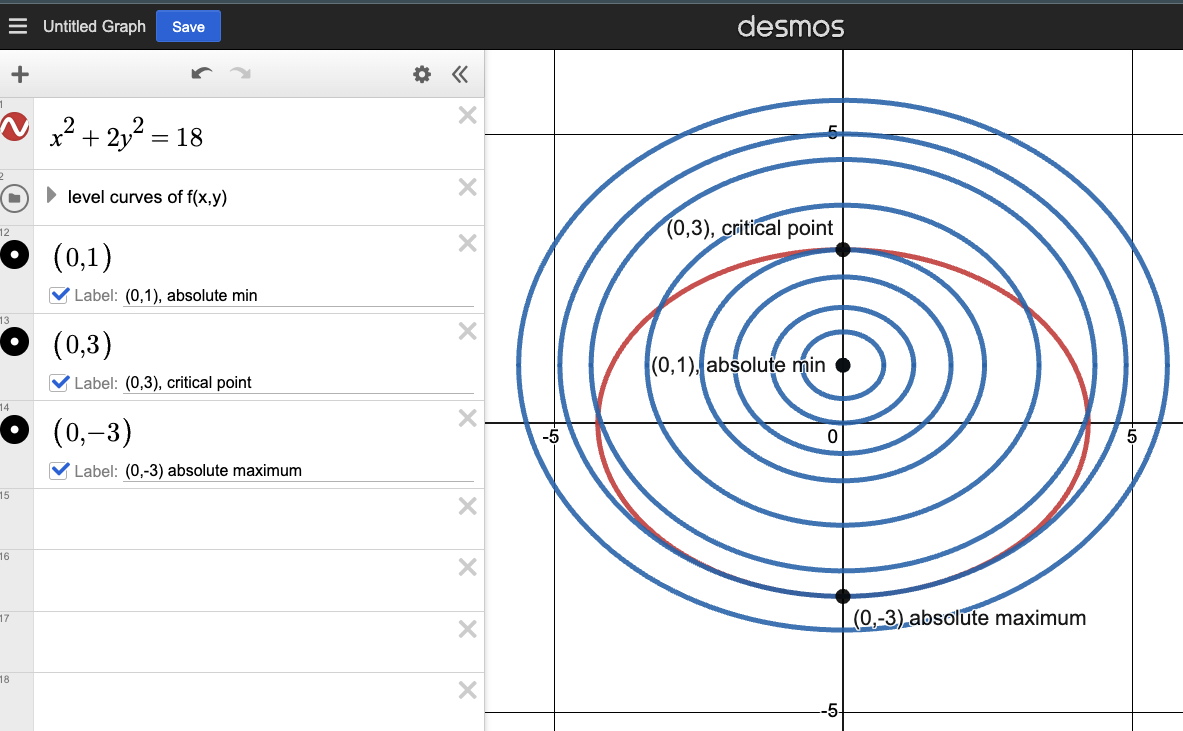
\includegraphics[width=0.95\textwidth]{202402/Exam2/Images/LagrangeCritPoints.png}
    \end{center}
    \end{itemize}    
    
    } 
   \else
      
   \fi
    
\fi

\ifnum \Version=8

    \question[6] Identify the maximum and minimum values of the function $f(x,y) = 4x - x^2 + 2y - y^2  + 4$ on the disk $x^2+y^2 \le 5$. Also determine where the extreme values are located. Please show your work. 
    \ifnum \Solutions=1 {\color{DarkBlue} \\ \textit{Solutions:} The partials we need are: 
    \begin{align*}
        f_x = 4 - 2x &=0 \ \quad \Rightarrow \quad x= 2 \\
        f_y = 2 - 2y &=0 \ \quad \Rightarrow \quad y= 1 
    \end{align*}
    There is a critical point at $(2,1)$, which happens to be on the boundary of the disk. Along the boundary using Lagrange Multipliers, set $g = x^2 + y^2 - 5 = 0$, assuming the origin is not a critical point,
    \begin{align*}
        \nabla f &= \lambda \nabla g \\
        \begin{pmatrix} 4 - 2x \\ 2 - 2y \end{pmatrix} &= \lambda \begin{pmatrix} 2x\\2y \end{pmatrix} \\ 
        \begin{pmatrix} 2 - x \\ 1 - y \end{pmatrix} &= \lambda \begin{pmatrix} x\\y \end{pmatrix} \\ 
        \begin{pmatrix} 2 \\ 1 \end{pmatrix} &= \begin{pmatrix} \lambda x + x\\ \lambda y + y \end{pmatrix} \\ 
        \begin{pmatrix} 2 \\ 1 \end{pmatrix} &= \begin{pmatrix} x(1 + \lambda )\\  y( 1 + \lambda) \end{pmatrix} \\ 
        x&=\frac{2}{1+\lambda} \\
        y&=\frac{1}{1+\lambda}
    \end{align*}
    Substitute into constraint: 
    \begin{align*}
        5 &=\left(\frac{2}{1+\lambda}\right)^2 + \left(\frac{1}{1+\lambda}\right)^2 \\
        5(1+\lambda)^2 &= 5 \\
        1 + \lambda &= \pm 1 \\
        \lambda = 0, -2
    \end{align*}
    When $\lambda = 0$, we get $(2,1)$, and when $\lambda = -2$ we get the point $(-2,-1)$. 
    Evaluate $f(x,y)$ at all critical points:
    \begin{align*}
        f(x,y) &= 4x - x^2 + 2y - y^2  + 4\\
        f(2,1) &= 4\cdot 2 - 2^2 + 2\cdot1 - 1^2+4 = 9 \ (\textbf{max})\\
        f(-2,-1) &= 4\cdot (-2) - (-2)^2 + 2\cdot(-1) - (-1)^2+4 = -11 \ (\textbf{min})
    \end{align*}
    \textbf{An Alternate Approach}\\
    The above approach is sufficient. But we could also use a parameterization of boundary to determine the max/min values of $f(x,y)$ on the boundary. One such parameterization would be $$x = k\cos t, \quad y = k\sin t, \ k = \sqrt5$$
    After substituting these expressions into $f(x,y)$, we would obtain a function of $t$ only, which we could differentiate, set to zero, and solve for $t$. This alternate approach would give us the min/max on the boundary of the region, which we could use instead of Lagrange multipliers. 
    } 
   \else
   \fi

\fi 






\ifnum \Version=9

    \question[6] Identify the maximum and minimum values of the function $f(x,y) = 4x - x^2 + 2y - y^2  + 4$ on the disk $x^2+y^2 \le 5$. Also determine where the extreme values are located. Please show your work. 
    \ifnum \Solutions=1 {\color{DarkBlue} \\ \textit{Solutions:} The partials we need are: 
    \begin{align*}
        f_x = 4 - 2x &=0 \ \quad \Rightarrow \quad x= 2 \\
        f_y = 2 - 2y &=0 \ \quad \Rightarrow \quad y= 1 
    \end{align*}
    There is a critical point at $(2,1)$, which happens to be on the boundary of the disk. Along the boundary using Lagrange Multipliers, set $g = x^2 + y^2 - 5 = 0$, assuming the origin is not a critical point,
    \begin{align*}
        \nabla f &= \lambda \nabla g \\
        \begin{pmatrix} 4 - 2x \\ 2 - 2y \end{pmatrix} &= \lambda \begin{pmatrix} 2x\\2y \end{pmatrix} \\ 
        \begin{pmatrix} 2 - x \\ 1 - y \end{pmatrix} &= \lambda \begin{pmatrix} x\\y \end{pmatrix} \\ 
        \begin{pmatrix} 2 \\ 1 \end{pmatrix} &= \begin{pmatrix} \lambda x + x\\ \lambda y + y \end{pmatrix} \\ 
        \begin{pmatrix} 2 \\ 1 \end{pmatrix} &= \begin{pmatrix} x(1 + \lambda )\\  y( 1 + \lambda) \end{pmatrix} \\ 
        x&=\frac{2}{1+\lambda} \\
        y&=\frac{1}{1+\lambda}
    \end{align*}
    Substitute into constraint: 
    \begin{align*}
        5 &=\left(\frac{2}{1+\lambda}\right)^2 + \left(\frac{1}{1+\lambda}\right)^2 \\
        5(1+\lambda)^2 &= 5 \\
        1 + \lambda &= \pm 1 \\
        \lambda = 0, -2
    \end{align*}
    When $\lambda = 0$, we get $(2,1)$, and when $\lambda = -2$ we get the point $(-2,-1)$. 
    Evaluate $f(x,y)$ at all critical points:
    \begin{align*}
        f(x,y) &= 4x - x^2 + 2y - y^2  + 4\\
        f(2,1) &= 4\cdot 2 - 2^2 + 2\cdot1 - 1^2+4 = 9 \ (\textbf{max})\\
        f(-2,-1) &= 4\cdot (-2) - (-2)^2 + 2\cdot(-1) - (-1)^2+4 = -11 \ (\textbf{min})
    \end{align*}
    } 
   \else
   \fi

\fi 







\ifnum \Version=10
\question[6] Identify the absolute maximum and minimum values of the function $f(x,y) = 2x^2 + 3y^2 - 6y$ on the region $x^2+2y^2 \le 18$, and determine where they are located. Please show your work. 
\ifnum \Solutions=1 {\color{DarkBlue} \\ \textit{Solutions:} For the interior the partials we need are: 
\begin{align*}
    f_x = 4x &=0 \ \quad \Rightarrow \quad x= 0 \\
    f_y = 6y -6 &=0 \ \quad \Rightarrow \quad y= 1 
\end{align*}
There is a critical point at $(0,1)$. Along the boundary using Lagrange Multipliers, set $g = x^2 + y^2 - 19 = 0$, and $\nabla f = \lambda \nabla g$ yields
\begin{align}
        \begin{pmatrix} 4x \\ 6y-6 \end{pmatrix} 
        &= \lambda \begin{pmatrix} 2x\\4y \end{pmatrix} 
    \end{align}
    The first component yields
    \begin{align}
        4x &= 2\lambda x
    \end{align}
    Either $\lambda =2$ or $x=0$. 
    \begin{itemize}
        \item \textbf{Case 1, $\lambda =2$}: the second components of the gradient equation yields
        \begin{align}
            6y-6 &= 4\lambda y = 8y\\
            2y &= -6
        \end{align} which implies $y = -3$. The constraint gives us values of $y$: 
        \begin{align}
            x^2 + 2y^2 &= 18 \\ 
            x^2 + 2(-3)^2 &= 18 \\ 
            x^2 &= 0
        \end{align}
        There is a critical point at $(0,-3)$.
        \item \textbf{Case 2, $x=0$}: the constraint gives us that 
        \begin{align}
            0^2+2y^2 = 18 \ \Rightarrow \ y = \pm 3
        \end{align}
        There are critical points at $(0, \pm 3)$. 
    \end{itemize}
    Evaluating $f$ at critical points: 
    \begin{align}
        f(x,y) &= 2x^2 + 3y^2 - 6y\\
        f(0,1) &= 0 + 3\cdot 1 - 6\cdot 1 = 3 - 6 = -3 \ (\textbf{min})\\ 
        f(0,3) &= 2\cdot 0 + 3\cdot 9 - 6\cdot(3)  = 27 - 18 = 9\\
        f(0,-3) &= 2\cdot 0 + 3\cdot 9 - 6\cdot(-3) = 27 + 18 = 45 \ (\textbf{max})
    \end{align}
    } 
   \else
      
   \fi
    
\fi






\ifnum \Version=11

    \question[6] Identify the maximum and minimum values of the function $f(x,y) = 4x - x^2 + 2y - y^2  + 4$ on the disk $x^2+y^2 \le 5$. Also determine where the extreme values are located. Please show your work. 
    \ifnum \Solutions=1 {\color{DarkBlue} \\ \textit{Solutions:} The partials we need are: 
    \begin{align*}
        f_x = 4 - 2x &=0 \ \quad \Rightarrow \quad x= 2 \\
        f_y = 2 - 2y &=0 \ \quad \Rightarrow \quad y= 1 
    \end{align*}
    There is a critical point at $(2,1)$, which happens to be on the boundary of the disk. Along the boundary using Lagrange Multipliers, set $g = x^2 + y^2 - 5 = 0$, assuming the origin is not a critical point,
    \begin{align*}
        \nabla f &= \lambda \nabla g \\
        \begin{pmatrix} 4 - 2x \\ 2 - 2y \end{pmatrix} &= \lambda \begin{pmatrix} 2x\\2y \end{pmatrix} \\ 
        \begin{pmatrix} 2 - x \\ 1 - y \end{pmatrix} &= \lambda \begin{pmatrix} x\\y \end{pmatrix} \\ 
        \begin{pmatrix} 2 \\ 1 \end{pmatrix} &= \begin{pmatrix} \lambda x + x\\ \lambda y + y \end{pmatrix} \\ 
        \begin{pmatrix} 2 \\ 1 \end{pmatrix} &= \begin{pmatrix} x(1 + \lambda )\\  y( 1 + \lambda) \end{pmatrix} \\ 
        x&=\frac{2}{1+\lambda} \\
        y&=\frac{1}{1+\lambda}
    \end{align*}
    Substitute into constraint: 
    \begin{align*}
        5 &=\left(\frac{2}{1+\lambda}\right)^2 + \left(\frac{1}{1+\lambda}\right)^2 \\
        5(1+\lambda)^2 &= 5 \\
        1 + \lambda &= \pm 1 \\
        \lambda = 0, -2
    \end{align*}
    When $\lambda = 0$, we get $(2,1)$, and when $\lambda = -2$ we get the point $(-2,-1)$. 
    Evaluate $f(x,y)$ at all critical points:
    \begin{align*}
        f(x,y) &= 4x - x^2 + 2y - y^2  + 4\\
        f(2,1) &= 4\cdot 2 - 2^2 + 2\cdot1 - 1^2+4 = 9 \ (\textbf{max})\\
        f(-2,-1) &= 4\cdot (-2) - (-2)^2 + 2\cdot(-1) - (-1)^2+4 = -11 \ (\textbf{min})
    \end{align*}
    } 
   \else
   \fi

\fi 


